% Reisgids Rome A5-booklet
\documentclass[10pt,twoside,a5paper]{article}
\usepackage[utf8]{inputenc}
\usepackage[T1]{fontenc}
\usepackage[dutch]{babel}
\usepackage{lmodern}
\usepackage{textcomp}
\usepackage{graphicx}
\usepackage[margin=18mm,headsep=8mm,includeheadfoot]{geometry}
\usepackage{parskip}
\usepackage{hyperref}
\hypersetup{colorlinks=true, linkcolor=black, urlcolor=blue}
\usepackage{enumitem}
\setlist[itemize]{nosep,left=0pt,label=--}
\usepackage{titlesec}
\titleformat{\section}{\normalfont\Large\bfseries}{\thesection}{1em}{}
\titleformat{\subsection}{\normalfont\bfseries}{\thesubsection}{1em}{}
\pagestyle{plain}
\begin{document}
\begin{titlepage}
  \thispagestyle{empty}
  \vspace*{8mm}
  \noindent
\includegraphics[width=0.28\textwidth]{logo.png}
  \vspace{10mm}
  \begin{center}
    {\Huge\bfseries Studiereis Rome}\\[3mm]
    {\Large Maandag 26 oktober t/m zondag 1 november 2026}\\[8mm]
    \hrule height 1pt
    \vspace{8mm}
    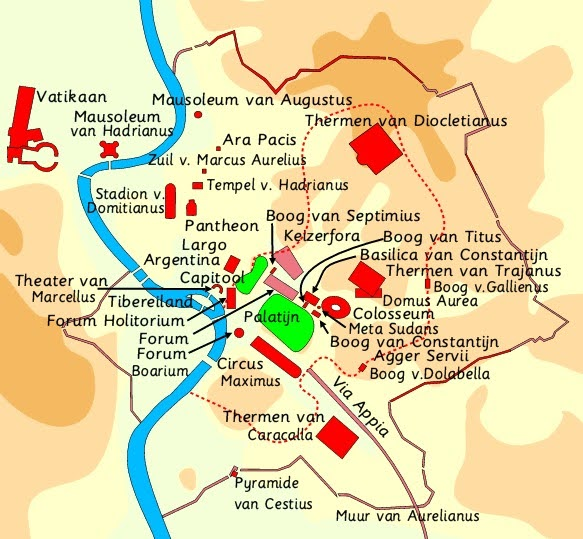
\includegraphics[width=0.88\textwidth,height=0.42\textheight,keepaspectratio]{kaartjeRome.jpg}\\[8mm]
    \hrule height 1pt
    \vspace{8mm}
    {\large \textit{Praktische reisinformatie voor leerlingen}}\\[2mm]
    {\large Villa Benedetta -- Rome}
  \end{center}
  \vfill
\end{titlepage}
\section*{Belangrijke info}
\subsection*{Heenreis}
Zorg dat je op maandag 26 oktober om 12:45 uur aanwezig bent bij scholengemeenschap Sint Ursula in Horn.
Bij het betreden van de bus controleren wij twee dingen:
\begin{itemize}
  \item Heb je een geldig reisdocument bij je?
  \item Heb je een envelop bij je met daarop je naam en erin 20 euro in contanten? Deze euro's zijn nodig als borg in het hotel in Rome en je krijgt ze terug als je je kamer onbeschadigd achterlaat.
\end{itemize}
Het is verstandig om eventuele beschadigingen in je kamer meteen te melden!
\begin{itemize}
  \item maandag 26 oktober, 13:00 uur: vertrek per touringcar vanaf Sint Ursula
  \item dinsdag 27 oktober, ca. 09:30 uur: aankomst in Rome
\end{itemize}

\subsection*{Terugreis}
Op zaterdagavond controleren we alle kamers op beschadigingen. Je moet je kamer ontruimen: we vertrekken deze avond terug naar Horn. Let op: tijdens de reis kun je niet meer aan je koffer!
\begin{itemize}
  \item zondag 1 november, ca. 17:00 uur: aankomst in Horn
\end{itemize}

\section*{Reis}
Je hebt een geldig paspoort of een geldige Europese identiteitskaart nodig. Bij het betreden van de bus wordt gecheckt of je dit document bij je hebt.
Je bagage wordt vervoerd onder in de bus: je kunt tijdens de reis niet in je koffer. Doe zaken die je onderweg nodig hebt daarom in je handbagage.
Liever geen al te grote koffers, liever geen ``harde'' koffers. Handbagage moet in het rek boven je stoel passen.

Bij aankomst in Rome stallen we onze bagage in het hotel. Daarna gaan we kennismaken met Rome. Gelukkig heb je goed geslapen, dus dat zal geen probleem zijn. In ieder geval bezoeken we meteen het verzamelpunt bij noodgevallen.

\textbf{Verzamelpunt bij noodgevallen (in je telefoon zetten):}
\begin{itemize}
  \item De fontein van de dikke Mozes (Largo Santa Susanna)
\end{itemize}

\section*{Programma}
\subsection*{Dinsdag}
\begin{itemize}
  \item Ochtend: aankomst bij het hotel nabij metrostation Ostiense en start van het programma te voet vanaf het hotel met de Aureliaanse muur en lunch in de omgeving.
  \item Middag: bezoek aan de thermen van Caracalla. Wandeling via de Celio / Celimontana (met gezicht op het Colosseum) langs het Circus Maximus. Bezoek aan het forum, de Palatijn en het Capitool. Vervolgens wandeling langs het theater van Marcellus (Marcello), de Tiber en eindigen in het ghetto.
  \item Avond: bezoek aan het Piazza Navona en eten in de buurt van het hotel.
\end{itemize}

\subsection*{Woensdag}
\begin{itemize}
  \item Ochtend: route langs de Sint-Pieter, Teutonico, de Friezen en de Engelenburcht.
  \item Middag: bezoek aan Santa Sabina / Aventijn, daarna nog niet ingevuld.
  \item Avond: bezoek aan de Pincio.
\end{itemize}

\subsection*{Donderdag}
\begin{itemize}
  \item Overdag (hoofdgroep): dagtocht naar Pompei.
  \item Overdag (programma voor de overgebleven leerlingen): dagtocht naar Ostia + strand.
  \item Avond: avondprogramma met de 10 leerlingen: bijvoorbeeld pizza eten en bowlen in de wijk Ostiense/Testaccio.
\end{itemize}

\subsection*{Vrijdag}
\begin{itemize}
  \item Ochtend: bezoek aan het Capitolijns museum.
  \item Middag: keuzeprogramma.
  \item Avond: avondprogramma in Trastevere.
\end{itemize}

\subsection*{Zaterdag}
\begin{itemize}
  \item Ochtend: uitchecken bij het hotel. Bezoek aan San Paolo en aansluitend met de metro naar het Marsveld.
  \item Middag: bezoek aan San Giovanni / Scala Santa, Santa Maria Maggiore / Santa Prassede en de Serviaanse muur / Termini.
  \item Avond: bezoek aan de Trevi-fontein als afsluiting, waarna vertrek vanaf Termini voor de terugreis naar Nederland.
\end{itemize}

\section*{Hotel}
Villa Benedetta Kloosteraccommodatie\\
Via della Moletta 10

\section*{Reisbureau}
Authentic Italia: \url{https://www.authentic-italia.nl/}

\section*{Begeleiders}
\begin{itemize}
  \item R. Menting \qquad +31 6 51 56 48 65
  \item H. Wieldraaijer \qquad +31 6 30 63 98 10
\end{itemize}

\textbf{Contactpersoon op school}
\begin{itemize}
  \item E. Nevels \qquad +31 6
\end{itemize}

\section*{Elke dag bij je hebben!!}
Goede wandelschoenen zijn een must. Niet alleen loop je veel, ook de straatstenen in Rome (de zogenaamde sanpietrini) zijn funest voor minder stevige schoenen.

Het kan nog warm zijn in deze tijd van het jaar, maar het kan ook regenen. In kerken is kleding die knieën en schouders bedekt verplicht. Als dat bij jouw knieën en/of schouders niet het geval is, stop dan een omslagdoek in je bagage! Niet ter plaatse gaan kopen.

Ook heb je altijd bij je: een kaartje van de heuvels van Rome en een tijdbalk van de geschiedenis van Rome. Dit krijg je van ons op een A4.

Indien nodig heb je altijd een gesloten envelop bij je met alle relevante informatie over medicijnen en dieetvoorschriften. Deze envelop wordt alleen geopend als dat noodzakelijk is, anders ongeopend terug. Voor sommige medicijnen is een Schengenverklaring nodig. Dieetwensen tijdig doorgeven.

\section*{Zakgeld}
Ontbijt, openbaar vervoer en entrees zijn inbegrepen bij de reis. Het zakgeld is onder andere voor je eten in de middag en de avond en wat te drinken.

\section*{Groepsindeling}
We zijn steeds met één groep en twee begeleiders, behalve tijdens de reis naar Pompeii of Ostia en tijdens het keuzeprogramma op vrijdagmiddag.

\section*{Rechten en plichten}
Zoals overal heb je rechten en plichten. Je hebt recht op een goede organisatie van de reis, binnen de grenzen van wat menselijkerwijs mogelijk is. De reis wordt inhoudelijk ook vakkundig en enthousiast geleid.

Gedurende de hele reis gelden de schoolregels. Dit houdt onder andere in dat alcohol verboden is. Natuurlijk veroorzaken we geen overlast in het hotel en houden we rekening met andere gasten.

Je mag niet alleen op stap: Rome is een moderne miljoenenstad met alle bijbehorende problemen. Dus altijd minstens met zijn drieën.

Onaangepast gedrag kan ernstige gevolgen hebben voor de hele groep. Je zult ontdekken dat begeleiders minder relaxt reageren dan op school. In het uiterste geval bellen we je ouders en sturen we je op eigen kosten terug naar Nederland.

\section*{Kopie ID}
Installeer thuis de KopieID-app en zorg dat je een kopie van je ID-kaart in deze app op je telefoon hebt staan.

\section*{Verzekering}
We hebben een annuleringsverzekering afgesloten voor de hele groep; deze verzekering betaalt niet uit aan individuele reizigers. Omdat de meeste mensen een doorlopende reisverzekering hebben, sluiten we die niet af. Dure spullen moet je dus zelf bijverzekeren of, nog beter, thuis laten. Laat kostbare spullen niet achter in de bus of in het hotel en houd ze goed in de gaten op drukke plaatsen en in het openbaar vervoer.

En als je vast wat Italiaans wil leren: probeer de apps Memrise of Duolingo.

\vfill
\begin{center}
  \textit{Buon viaggio!}
\end{center}
\end{document}
